\documentclass[a4paper]{article}
\usepackage[top=1cm, bottom=1cm, left=2.5cm, right=1cm]{geometry}


\usepackage{amssymb}
\usepackage{euscript}
\usepackage{graphicx}
\graphicspath{{pics/}}
\usepackage{color}
\usepackage{epsfig}
\textwidth=18cm
\renewcommand{\arraystretch}{1.2}
\renewcommand{\tabcolsep}{1mm}

\begin{document}

\hrule
\subsection*{{\tt sig\_freq} --- processing magnon condensate signals\\
for free surface measurements\\
with forced cryostat oscillations}
\hrule
\bigskip

\medskip\noindent{\bf Location:} {\tt /rota/Analysis/PS/osc2011}

\medskip\noindent{\bf Important assumptions:}
\begin{itemize}
\item Exitation signal (from geophone sensor) in the 1st channel.
\item Magnon condensate signal in the 2nd channel.
\item Phrase ``exc[...]g[...]Hz'' in the signal name with excitation gain and (non-zero) frequency.
\item Signal averaging is not supported.
\end{itemize}

If filename is ``test'' than model signal is used.

\medskip\noindent{\bf Parameters:}

All {\tt sig\_read} parameters except {\tt chan}:\\
{\tt t0}, {\tt t1}, {\tt t2}, {\tt auto0}, {\tt auto0th}, {\tt auto0st}.

All {\tt sig\_trace} parameters:\\
{\tt fmin} or {\tt minf}, {\tt fmax} or {\tt maxf},
{\tt window}, {\tt step}, {\tt f0}, {\tt df}, {\tt ftracer}, {\tt fix\_lock\_in}.

\medskip\noindent
\begin{tabular}{p{3cm}p{1cm}p{13cm}}\hline
\bf name & \bf def & \bf description\\
df      & 100 & Filtering range (also used in {\tt sig\_trace})\\
smin    & 2   & Minimal frequency for signal frequency and excitation spectra.\\
smax    & df  & Maximal frequency for signal frequency and excitation spectra.
                Values greater then df are usless.\\
exc\_df & 1   & Frequency half-range (Hz) for excitation and frequency peak integration.
                Also used to adjust excitation frequncy to the near maxinum.
                Also used to filter excitation signal for lock-in calculations.\\
\hline
\end{tabular}
\medskip

These parameters are not saved in cache:

\medskip\noindent
\begin{tabular}{p{3cm}p{1cm}p{13cm}}\hline
\bf name & \bf def & \bf description\\
do\_plot   & 1    & Plot figure \\
list\_file & ``'' & Used in list file processing \\
refit      & 0    & Force processing, don't use cache.\\
usecache   & 0    & Skip processing, use cache even if it is outdated\\
save\_freq\_txt & ``'' & Save frequency spectrum to a txt file\\
\hline
\end{tabular}
\medskip

\medskip\noindent{\bf Processing:}

\begin{itemize}
\item Read signal (channel 2) and excitation (channel 1) data.
\item Do usual sliding fft and frequency tracing of the signal.
\item Filter signal in {\tt min(freq)-df .. max(freq)+df} range.
\item Use filtered signal zeros to find frequency. Select largest
      range where frequency is inside filtering range.
\item Parse signal name to get excitation frequency ({\tt exc\_fre0}).
      Find excitation maximum in the {\tt exc\_fre0}$\pm${\tt exc\_df} range,
      {\tt exc\_fre} and {\tt exc\_amp} values.
\item Calculate excitation peak integral {\tt exc\_int}$=\sqrt{\int A^2\ df}$
      in {\tt exc\_fre}$\pm${\tt exc\_df} range. Filter excitation signal
      in the same range.
\item Do lock-in calculation at 1x and 2x {\tt exc\_fre}: multiply signal
      frequency by 1st and 2nd power of filtered excitation signal with
      appropriate phase shifts and scales.
\item Calculate integrals of signal frequency spectrum near 1x and 2x{\tt exc\_fre}.
\end{itemize}
\medskip

\medskip\noindent{\bf Results:}

Structure with following fields is returned:

\medskip\noindent
\begin{tabular}{p{3cm}p{14cm}}\hline
\tt exc\_fre0  & excitation frequency (from filename)\\
\tt exc\_gain  & excitation gain (from filename)\\
\tt exc\_fre   & measured excitation freq (peak maximum)\\
\tt exc\_amp   & measured excitation amplitude (peak maximum)\\
\tt exc\_int   & integral of the excitation F peak\\
\tt sig\_int1  & integral of signal frequncy 1xF peak\\
\tt sig\_int2  & integral of signal frequncy 2xF peak\\
\tt sig\_lia1  & lock-in amplitude of 1xF peak (complex)\\
\tt sig\_lia2  & lock-in amplitude of 2xF peak (complex)\\
\tt pars\_read & parameters for {\tt sig\_read}\\
\tt pars       & other parameters\\
\tt cache      & was cache used or not\\
% specf
% speca
\hline
\end{tabular}
\medskip

\medskip\noindent{\bf Figure example:}

\medskip
\noindent
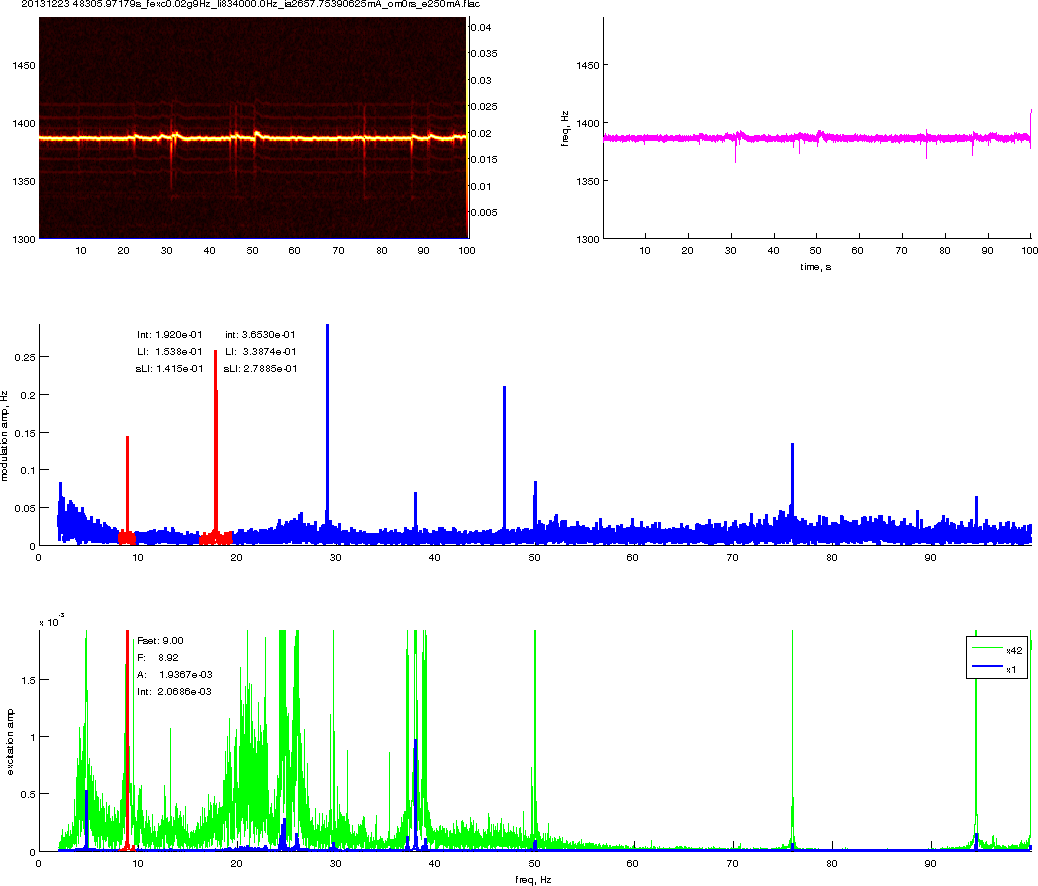
\includegraphics[width=\textwidth]{sig_freq}
\end{document}
